


\chapter{Numerical Results}
  \label{ch_results}

\todo{This chapter is the real moneymaker. The overarching motivation for this work is that Pc4 pulsations vary in interesting ways with respect to azimuthal modenumber, and that prior models have been unable to give a good picture of that behavior. }

%\todo{Do we every check E/B against $\Sigma_P / \mz$? }

%\todo{Do we see a difference between \vec{k} (momentum) and the group velocity? Poynting flux will always be pretty much along the field line, since $B_3$ is small and $E_3$ is zero, but the wave vector need not be. This is a question of coupling/converting to compressional waves, I guess. }

%\todo{Look at McKenzie and Westphal. Waves incident on the bow shock, etc, at weird angles. }

%\todo{Look at the E to B ratio. Compare to the \Alfven speed and to the height-integrated Pedersen conductivity. }

% -----------------------------------------------------------------------------
% -----------------------------------------------------------------------------
% -----------------------------------------------------------------------------
\section{Finite Poloidal Lifetimes}
  \label{sec_lifetimes}

In his 1974 paper, Radoski argues that a poloidally-polarized wave should asymptotically rotate to the toroidal polarization\cite{radoski_1974} as a result of the curved derivative in the meridional plane. The question of finite poloidal lifetimes is considered further in a 1995 paper by Mann and Wright\cite{mann_1995}. Their numerical work used a straightened field line, with an \Alfven speed gradient in the ``radial'' direction. They also found a rotation over time from poloidal to toroidal polarization, with the characteristic time proportional to the azimuthal modenumber. 

\todo{Ding et al\cite{ding_1995} did similar work just before Mann and Wright, but results were less clear, possibly due to issues with grid resolution (as discussed in \cite{mann_1995}). }

\todo{Mann and Wright looked specifically at second harmonics. This work is on first harmonics. (In principle Tuna allows arbitrary driving waveforms and spatial distributions.) }

The present section builds on the aforementioned results by relaxing several of their nonphysical assumptions. First, Tuna's geometry (as described in \cref{ch_model}) is far more realistic than Radoski's half-cylinder or the box model used by Mann and Wright. Magnetic field lines are dipolar. \Alfven speed is based on an empirical profile, and varies along and across field lines. Next, the present results feature driving delivered over time through perturbation of the ring current; past work has instead considered only the evolution of an initial condition. Finally, the present model includes a height-resolved ionosphere (rather than perfectly-reflecting boundaries). The ionospheric conductivity provides a direct coupling between the poloidal and toroidal modes, in addition to dissipating energy. 

Each subplot in \cref{fig_U_2_4_5,fig_U_2_5_5,fig_U_3_4_5,fig_U_3_4_6} is analogous to Mann's Figure 3. Blue lines show the total energy in the poloidal mode as a function of time. Red lines show toroidal energy. Runs are organized such that driving frequency is constant down each column, and azimuthal modenumer is constant across each row. Axis bounds are held constant across all subplots. 

Energy is computed per Poynting's theorem, with due consideration of the unusual geometry. Energy density is integrated over the meridional plane, but not in the azimuthal direction, giving units of gigajoules per radian; more than anything else, this serves as a reminder that the waves under consideration are azimuthally localized. 
\begin{align}
  \label{def_energy}
  U_P &= \displaystyle\int \frac{d\lysakx d\lysakz}{2 \mz \jac} \lr{ B_x^2 + \frac{1}{\va^2} E_y^2} &
  U_T &= \displaystyle\int \frac{d\lysakx d\lysakz}{2 \mz \jac} \lr{ B_y^2 + \frac{1}{\va^2} E_x^2} 
\end{align}

The twenty-eight runs shown in \cref{fig_U_2_4_5} use a high-conductivity profile, corresponding to the dayside with low solar activity. 

\begin{figure}[!htb]
    \centering
    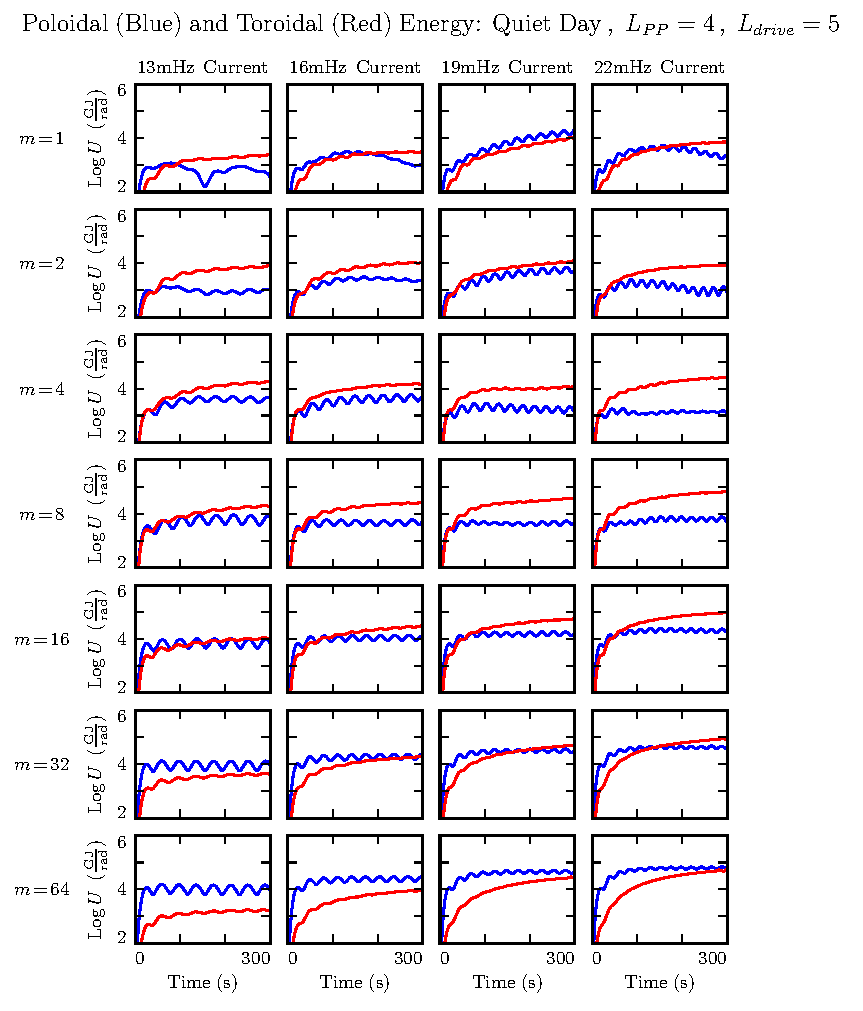
\includegraphics[width=\textwidth]{figures/U_2_4_5.pdf}
    \caption[Poloidal and Toroidal Energy: Quiet Day, Typical Plasmasphere]{
      Driving is continuously injected into the poloidal mode (energy in blue). The waves rotate asymptotically to the toroidal mode (red). When the azimuthal modenumber (rows) is large, the rotation is slower. The driving frequency (columns) also affects the asymptotic accumulation of energy. 
    }
    \label{fig_U_2_4_5}
\end{figure}


\begin{figure}[!htb]
    \centering
    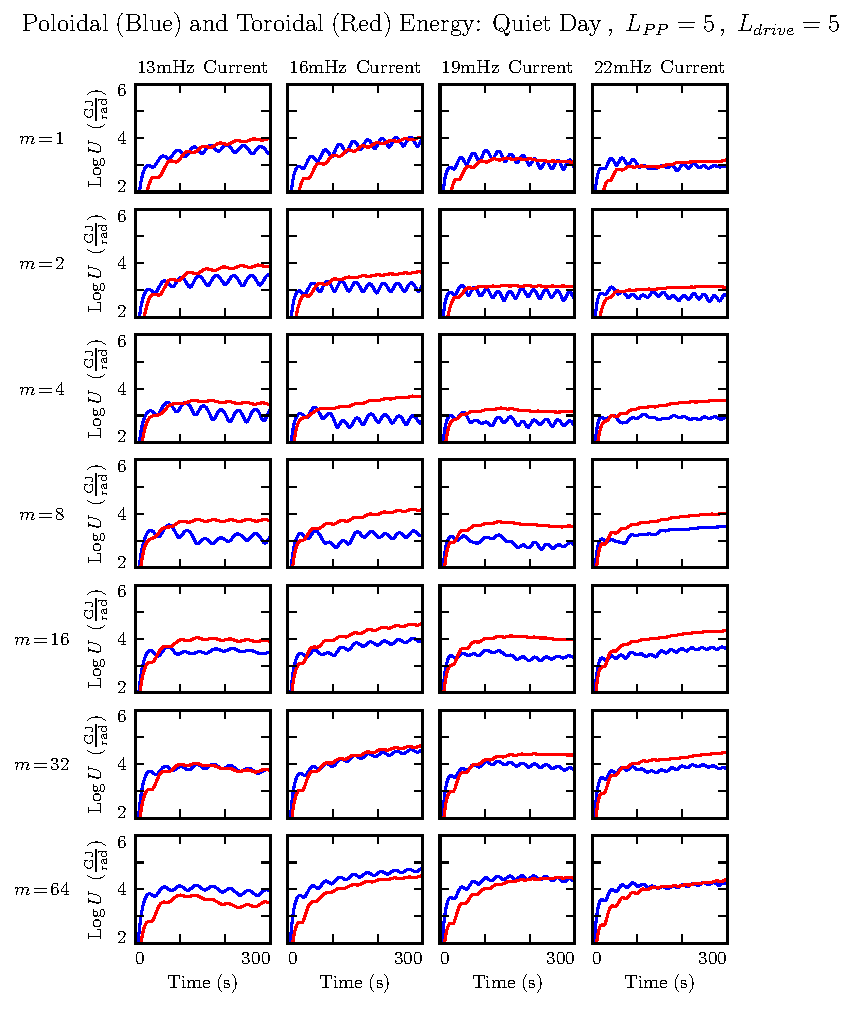
\includegraphics[width=\textwidth]{figures/U_2_5_5.pdf}
    \caption[Poloidal and Toroidal Energy: Quiet Day, Large Plasmasphere]{
      Above is a figure identical to \cref{fig_U_2_4_5}, except that the plasmapause has been moved from $L_{PP} = 4$ to $L_{PP} = 5$. This affects which driving frequency is closest to the resonant \Alfven frequency, and hence is most effective is causing a buildup of energy over time. 
    }
    \label{fig_U_2_5_5}
\end{figure}

The fact that red (toroidal) lines appear at all speaks to the coupling of the poloidal and toroidal modes. As discussed in \cref{ch_model}, driving in Tuna is delivered purely into the poloidal electric field (reflecting the azimuthal direction of the ring current). 

As predicted, the rotation from poloidal to toroidal is slowest at large azimuthal modenumbers. The toroidal energy overtakes the poloidal energy within a single drive period at $\azm=4$; with $\azm=64$, the most of the energy is in the poloidal mode for \about10 periods. However, the relationship between azimuthal modenumber and rotation timescale is not linear, as was suggested by Mann and Wright. Instead, the rotation is fastest at $\azm=4$. 

This hints at two competing effects, and there are only so many options. In addition to the poloidal-to-toroidal rotation, the two modes are coupled by the ionospheric Hall conductivity; energy is also is lost when waves propagate out of the simulation domain, and as a result of Joule dissipation. 

In practice, the Hall conductivity does not move large amounts of energy between the poloidal and toroidal modes. In fact, when the runs shown in \cref{fig_U_2_4_5} are repeated with Hall conductivity uniformy zero (not shown), the energy curves are not visibly distinct. 

Joule dissipation --- discussed further below --- is a major player in the simulation's energy economy, but does not depend directly on the azimuthal modenumber. 

That leaves the propagation of energy across field lines, which does explain the observed behavior. As the azimuthal modenumber increases past order unity, compressional \Alfven waves in the Pc4 band become evanescent\footnote{See \cref{sec_implications}. }. Runs in the top two rows lose considerable sums of energy as a result of waves propagating out of the simulation domain. In contrast, runs conducted at higher modenumber are not conducive to compressional \Alfven waves, so no energy escapes through the outer boundary. 

Notably, the low-modenumber runs at \SI{19}{\mHz} do accumulate significant energy over time, while those at \SI{13}{\mHz}, \SI{16}{\mHz}, and \SI{22}{\mHz} falter. This is because \SI{19}{\mHz} driving excites the third harmonic just inside the simulation's outer boundary. Coupling to the shear \Alfven wave at $L\about9$ gives energy a second chance to resonate before being lost to the outer boundary. 

In each run, the energy of the system is asymptotically determined by the balance between the energy input (from driving) and the energy loss (through Joule dissipation in the ionosphere, and, at low \azm, escape through the outer boundary). When the driving frequency matches closely with the local \Alfven frequency, energy accumulates over a number of drive periods, leading to a relatively large asymptotic energy in the system. 

The system's resonant frequency (for a fundamental poloidal mode at $L\about5$) is affected significantly by the size of the plasmasphere. In \cref{fig_U_2_4_5}, with the plasmapause at $L_{PP}=4$, the system resonates at \SI{19}{\mHz} at low \azm; as \azm becomes large, the resonant frequency is closer to \SI{22}{\mHz}. \cref{fig_U_2_5_5} shows the effect of moving the plasmapause to $L_{PP}=5$: resonance is closer to \SI{16}{\mHz}. The runs are otherwise identical to those shown in \cref{fig_U_2_4_5}. 

On the nightside, the picture changes significantly. 

\begin{figure}[!htb]
    \centering
    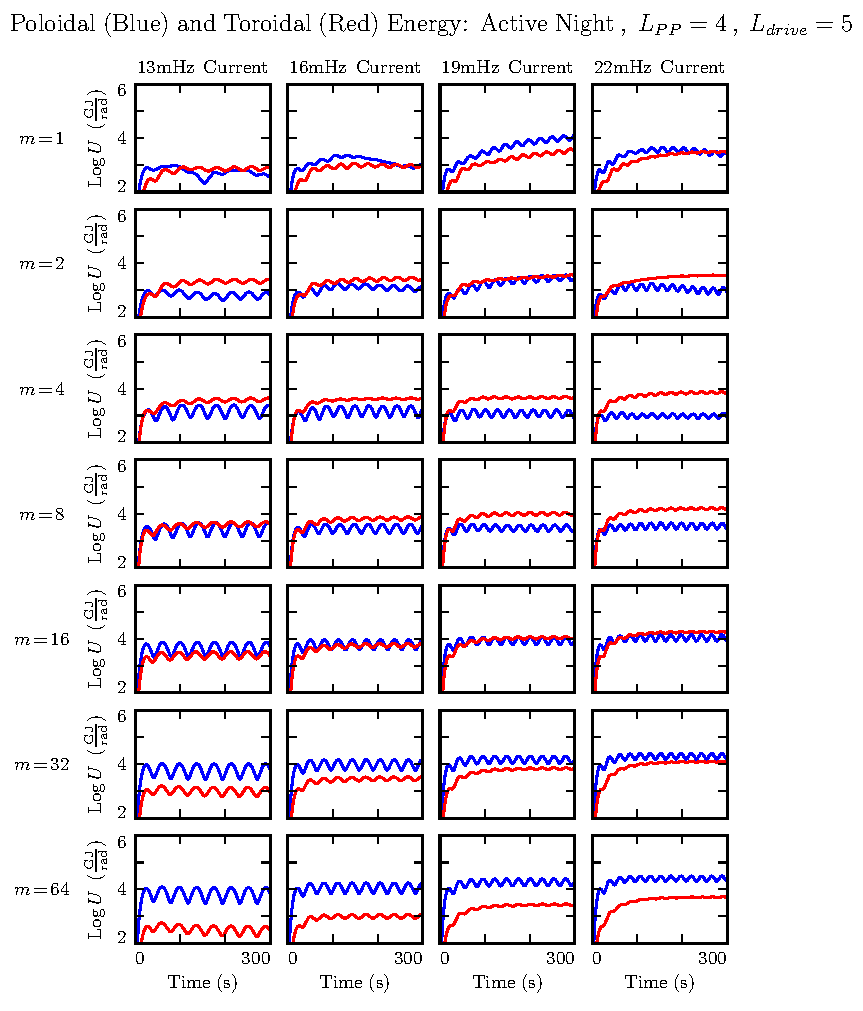
\includegraphics[width=\textwidth]{figures/U_3_4_5.pdf}
    \caption[Poloidal and Toroidal Energy: Active Night, Driving at $L=5$]{
      On the nightside, driving in the Pc4 band is not resonant at $L\about5$. This --- combined with the less-conductive ionosphere --- causes the poloidal (blue) and toroidal (red) energies to quickly reach their asymptotic values. As on the dayside, energy rotates from poloidal to toroidal most effectively at small-but-finite \azm. 
    }
    \label{fig_U_3_4_5}
\end{figure}

Due to the difference in electric constant between the dayside and nightside magnetospheres\footnote{See \cref{fig_fa}. }, resonant frequencies just outside the typical ($L_{PP} = 4$) plasmapause are well above the Pc4 range. As shown in \cref{fig_U_3_4_5}, this results in little energy accumulation across the board --- compared to \cref{fig_U_2_4_5}, where the driving was near the resonant frequency, asymptotic energies are lower on the nightside by an order of magnitude or more. 

Even so, the poloidal-to-toroidal rotation is qualitatively the same. The further the azimuthal modenumber from the rotation peak at $\azm = 4$, the lower the asymptotic toroidal energy level is compared to the poloidal. If anything, the effect is exaggerated by the small dissipation timescale. When $\azm = 64$, only \about\SI{1}{\percent} of the energy in the poloidal mode rotates to the toroidal mode before being lost. 

Behavior closer to resonance is shown in \cref{fig_U_3_4_6}. 

\begin{figure}[!htb]
    \centering
    
\includegraphics[width=\textwidth]{figures/placeholder.jpg}
    \caption[Poloidal and Toroidal Energy: Active Night, Driving at $L=7$]{
      \todo{Nightside with $L_{drive} = 7$. }
    }
    \label{fig_U_3_4_6}
\end{figure}

The results of the present section show agreement with --- and significant refinement of --- past analytical and numerical work. In the case of large (but finite) ionospheric conductivity, dipole geometry, and realistic \Alfven speed profile, energy rotates asymptotically from the poloidal mode to the toroidal mode. The rotation rate is strongly affected by azimuthal modenumber and, in the large-\azm regime, has a characteristic timescale in the tens of periods. 

\todo{The following may need to be reworked --- a few final attempts are currently running, to see if it's possible to get something nice looking on the nightside. }

The present work furthermore considers the issue of poloidal lifetimes in the low conductivity regime (while past work has used perfectly-reflecting boundaries). The result is novel: rather than asymptotically accumulating energy in the toroidal mode, an FLR on the nightside does not seem to accumulate energy at all. This is relevant to the question of day-night asymmetry in the observation of field line resonances. 

% -----------------------------------------------------------------------------
% -----------------------------------------------------------------------------
% -----------------------------------------------------------------------------
\section{Spatial Distribution of Energy}
  \label{sec_layers}

\todo{Maybe this section should go before the previous one? They sorta depend on one another. It's not clear if there's a better way to divide things up. }

Looking a bit deeper, it's possible to comment on the structure of the poloidal and toroidal modes, not just their magnitudes. The subplots in \cref{fig_layers_p_2_4_5,fig_layers_p_2_5_5,fig_layers_t_2_4_5} are arranged analogously to those in \cref{sec_lifetimes}: each comes from a different run, modenumber is held constant across each row, and frequency down each column. 

Contours represent energy density, averaged over the ``volume'' of a flux tube. The vertical axis shows $L$-shell, while the horizontal axis is time. As above, poloidal and toroidal energy density are computed separately. The qualitative differences between the contours in \cref{fig_layers_p_2_4_5} and those in \cref{fig_layers_t_2_4_5} showcase the different behaviors of the poloidal and toroidal FLR modes. 

\begin{figure}[!htb]
    \centering
    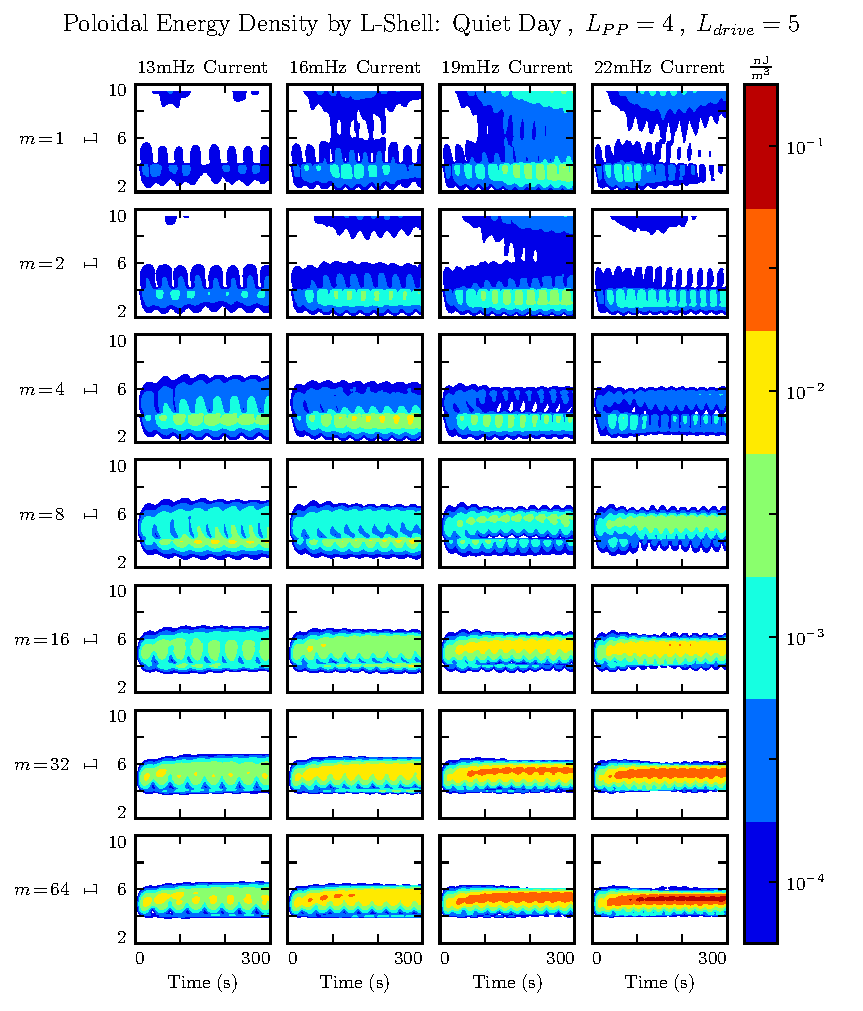
\includegraphics[width=\textwidth]{figures/layers_p_2_4_5.pdf}
    \caption[Radial Distribution of Poloidal Energy: Quiet Day, Typical Plasmasphere]{
      \todo{Explain figure?} At low \azm, the poloidal mode does not resonate effectively along a field line. Energy instead moves radially, and also rotates quickly to the toroidal mode. At high \azm, energy injected into the poloidal mode cannot move compressionally, and the mode rotation is slow, allowing a strong resonance --- but only when the driving frequency matches the local \Alfven frequency. 
    }
    \label{fig_layers_p_2_4_5}
\end{figure}

At low modenumber, the poloidal mode doesn't resonate effectively. Its coupling between the shear and compressional \Alfven waves allows energy to be spread broadly in $L$. Some energy builds up in a third harmonic resonance near the outer boundary (shown best in the \SI{19}{\mHz} run with $\azm = 1$). Some energy moves inward, and is trapped in the plasmapause's steep \Alfven speed gradient (particularly visible in the \SI{16}{\mHz}, $\azm = 4$ run). The time spent propagating across field lines counts against the poloidal mode's finite lifetime --- by the time a poloidally-polarized wave reaches the outer boundary, a significant fraction of its energy has rotated to the toroidal mode. 

The peak energy density in the bottom-right run (\SI{22}{\mHz} driving, $\azm = 64$) is by far the largest of any run in \cref{fig_layers_p_2_4_5}. The azimuthal modenumber is large, so the poloidal mode is purely guided; no time is wasted with movement across magnetic field lines. And, crucially, the frequency of the driving aligns closely with the resonant frequency where it's delivered. Other runs on the bottom row also have $\azm = 64$ (and so are also guided), but their driving frequencies do not align with the local resonant frequency, so they build up energy much less effectively. 

\begin{figure}[!htb]
    \centering
    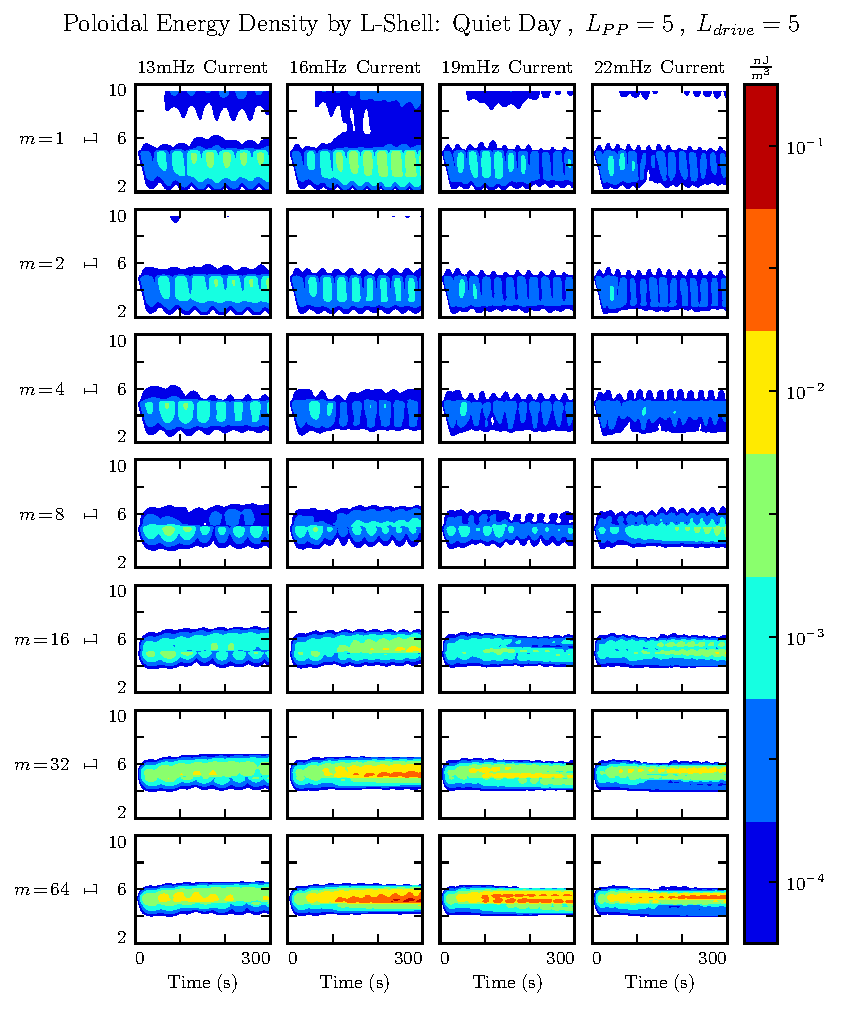
\includegraphics[width=\textwidth]{figures/layers_p_2_5_5.pdf}
    \caption[Radial Distribution of Poloidal Energy: Quiet Day, Large Plasmasphere]{
      \todo{Explain figure?} The \Alfven frequency is significantly affected by the size of the plasmasphere. The runs shown above are identical to those in \cref{fig_layers_p_2_4_5}, except that the plasmapause has been moved from $L_{PP} = 4$ to $L_{PP} = 5$. As a result, the most effective resonance at $L\about5$ is shifted from \SI{22}{\mHz} to \SI{16}{\mHz}. 
    }
    \label{fig_layers_p_2_5_5}
\end{figure}

Similar behavior can be seen in \cref{fig_layers_p_2_5_5} (which shows the same runs as \cref{fig_U_2_5_5}). A third harmonic resonance can be seen at the outer boundary for runs on the top row ($\azm = 1$). The effect of the plasmapause is particularly visible in the middle row, $\azm = 8$, where energy accumulates both just inside and just outside $L_{PP} = 5$. At high modenumber, the driving resonates best at \SI{16}{\mHz}; at other frequencies, energy density has a lower asymptotic value, which is reached more quickly. 

\begin{figure}[!htb]
    \centering
    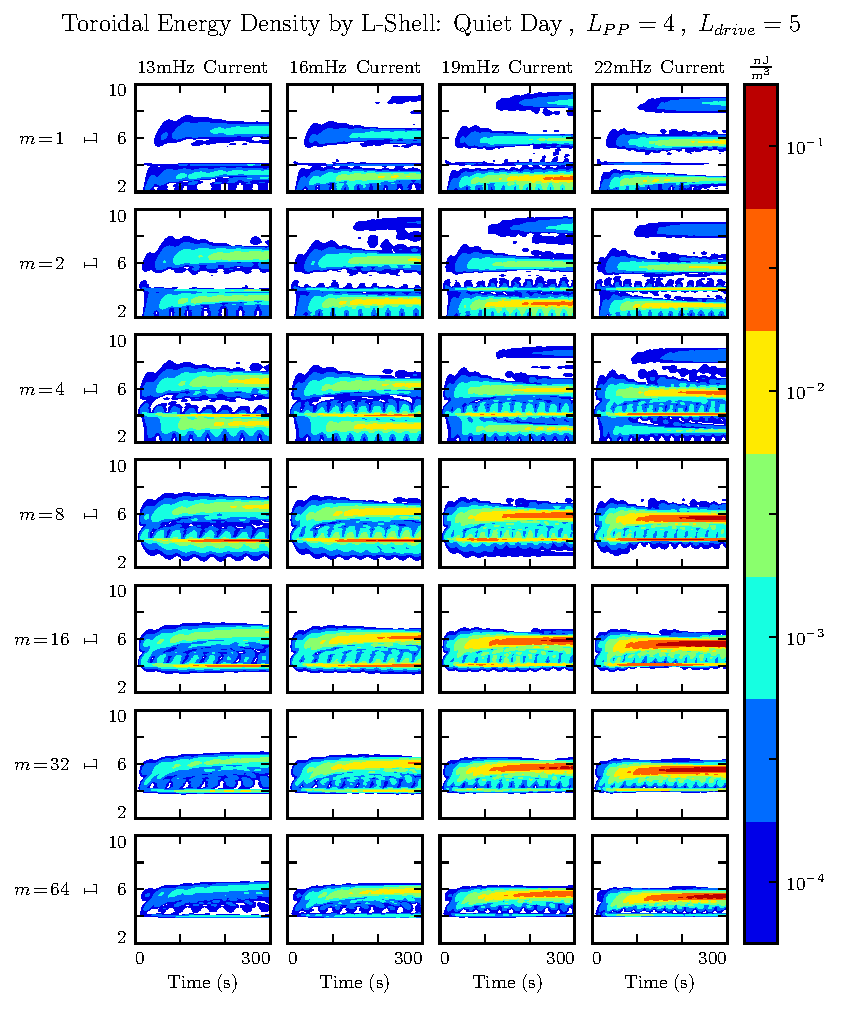
\includegraphics[width=\textwidth]{figures/layers_t_2_4_5.pdf}
    \caption[Radial Distribution of Toroidal Energy: Quiet Day]{
      \todo{$\cdots$}
    }
    \label{fig_layers_t_2_4_5}
\end{figure}

\todo{Talk about the toroidal mode. }

\begin{figure}[!htb]
    \centering
    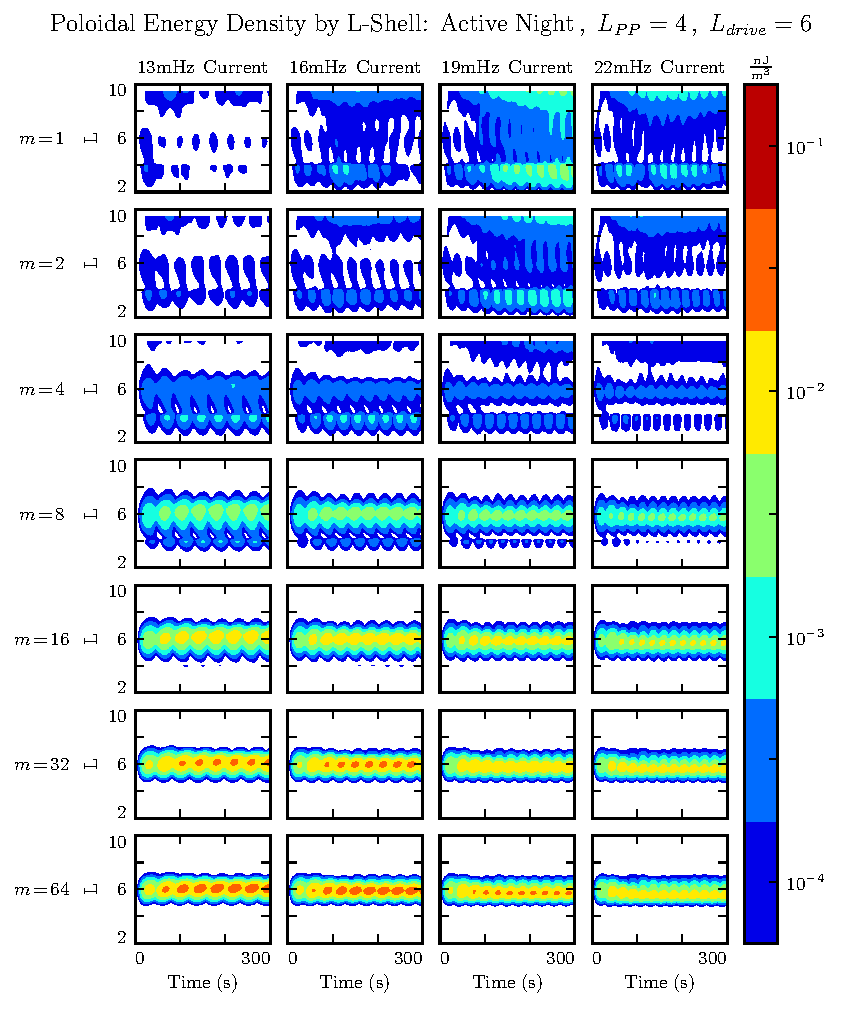
\includegraphics[width=\textwidth]{figures/layers_p_3_4_6.pdf}
    \caption[Radial Distribution of Poloidal Energy: Active Night]{
      \todo{Nightside poloidal, $L_{PP} = 4$ to $L_{PP} = 6$. }
    }
    \label{fig_layers_p_3_4_6}
\end{figure}

\begin{figure}[!htb]
    \centering
    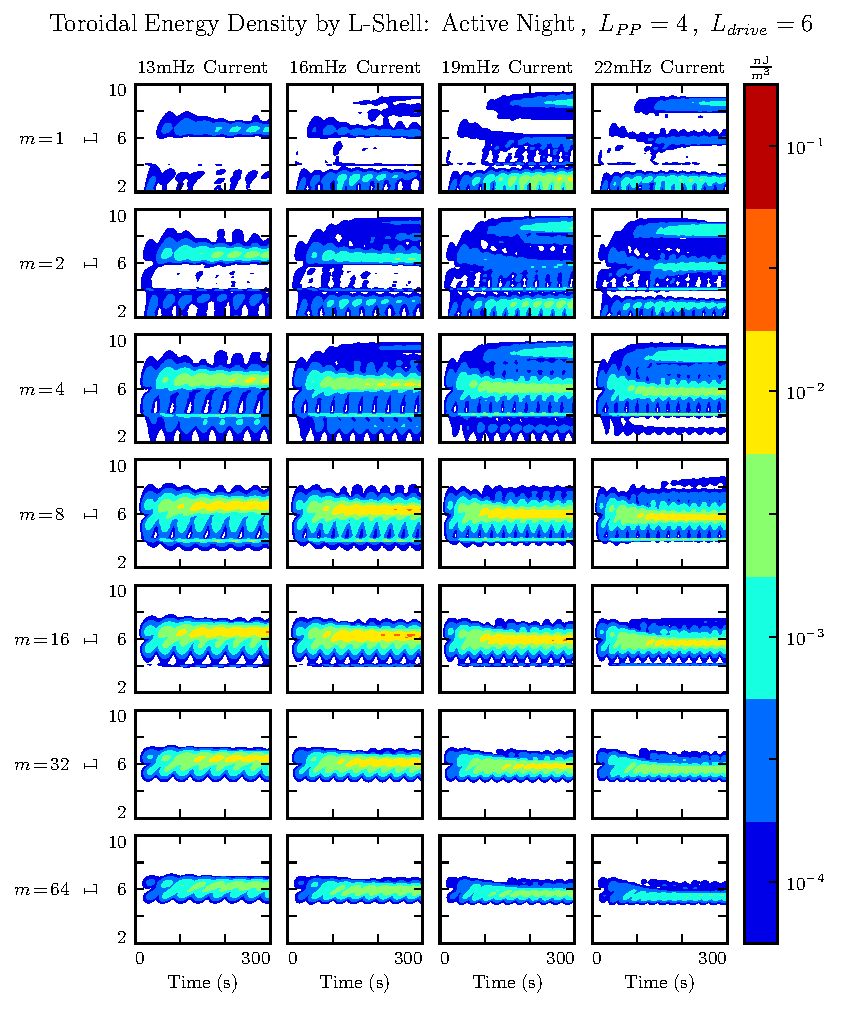
\includegraphics[width=\textwidth]{figures/layers_t_3_4_6.pdf}
    \caption[Radial Distribution of Toroidal Energy: Active Night]{
      \todo{Nightside toroidal, $L_{PP} = 4$ to $L_{PP} = 6$. }
    }
    \label{fig_layers_t_3_4_6}
\end{figure}

%\todo{If \azm is small, energy rotates to the toroidal mode too fast to form a poloidal resonance. If \azm is large, the \Alfven wave is guided, so it resonates only if the driving frequency lines up with the resonant frequency where it's applied. The result is just one big --- or perhaps even giant --- pulsation. If the driving lines up with a nearby field line, the toroidal mode goes crazy! Resonance inside the plasmasphere. Resonance at the plasmapause. Resonance at the driving location. And (weak) attempt at a higher harmonic further out. }

%\todo{When the driving frequency doesn't line up with the location where it's delivered, there's basically no response. There is no movement of energy to a resonant field line, so no energy can accumulate over the course of multiple rounds of driving. Even when not driven resonantly, the toroidal mode still makes the best of its situation. It steals what energy it can from the poloidal mode, carries it to the resonant $L$-shell, and gets to work. (In contrast, recall from \cref{fig_resonant_driving}, in this situation the poloidal mode just does not accumulate energy.) }

% -----------------------------------------------------------------------------
% -----------------------------------------------------------------------------
% -----------------------------------------------------------------------------
\section{Ground Signatures}

FLRs in space give rise to magnetic pulsations at Earth's surface. 

\todo{Rotation of about \SI{90}{\degree} due to passing through the ionosphere. }

\todo{Screening of large modenumbers. }

\todo{Ground signatures are distinguishable between active and quiet times, but the differences between dayside and nightside are much greater. }

\begin{figure}[!htb]
    \centering
    
\includegraphics[width=\textwidth]{figures/placeholder.jpg}
    \caption[Dayside Ground Magnetic Fields]{
      The east-west component of magnetic ground signatures is peaked on the geomagnetically quiet dayside, at modenumbers around 16 to 32. This coincides nicely with observations of giant pulsations. Like the east-west component, the north-south ground signature is strongest on the quiet dayside; however, unlike the east-west component, the north-south component is weak when the modenumber is large. 
    }
    \label{fig_ground_2_4_5}
\end{figure}

\begin{figure}[!htb]
    \centering
    
\includegraphics[width=\textwidth]{figures/placeholder.jpg}
    \caption[Nightside Ground Magnetic Fields]{
      \todo{Nightside ground signatures. }
    }
    \label{fig_ground_3_4_6}
\end{figure}


% -----------------------------------------------------------------------------
% -----------------------------------------------------------------------------
% -----------------------------------------------------------------------------
\section{Discussion}

... \\ \\ \\




Giant pulsations are (probably\cite{takahashi_2011}) fundamental mode poloidal Pc4 pulsations with frequencies around \SI{10}{\mHz} and azimuthal modenumbers around \num{20}. They are large, and can sometimes be observed on the ground. 

While this model makes no particular distinction between a giant pulsation and any other Pc4, the above results do line up with giant pulsation observations. 

Giant pulsations aren't seen at small \azm. As shown in \cref{sec_lifetimes}, low-\azm poloidal modes rotate to the toroidal mode too quickly to resonate effectively, even in the case of continuous driving at a locally-resonant frequency. The sweet spot seems to be around $\azm = 20$, more or less the same point where resonance becomes visible in \cref{fig_U_2_4_5}. Admittedly, giant pulsations are typically closer to \SI{10}{\mHz} than \SI{22}{\mHz}. It seems likely that qualitatively similar results would be encountered if the driving were moved to an $L$-shell with a bounce time of \SI{10}{\mHz}. 


\todo{Present profiles do not allow a distinction between the dawn and dusk flank. Future work... Tuna could easily accept new profiles! }


% GROUND SIGNATURES

\todo{\cite{takahashi_2011} talks significantly about the east-west polarization. }

Giant pulsations are seen at very large \azm, though not on the ground\cite{takahashi_2013}, due to damping by the ionosphere. 

Giant pulsations are most common on the dayside (particularly the morningside), during geomagnetically quiet times. Giant pulsation ground signatures are noted for their predisposition towards east-west polarization. 

In \cref{fig_ground_signatures}, the strongest east-west ground signatures is obtained on the geomagnetically quiet dayside, at \azm of 16 and 32. 

This seems to be a giant pulsation ``sweet spot'': the poloidal mode becomes stronger as \azm increases, but the ionospheric damping also increases. 

Giant pulsations are monochromatic, and can be accompanied by ``multiharmonic toroidal waves''\cite{takahashi_2011}. Per \cref{sec_layers}, this is about what would be expected from a mishmash of poloidal driving. Poloidal modes of all frequencies rotate into the toroidal mode; resonant poloidal modes resonate; non-resonant poloidal modes become evanescent. 

Giant pulsations often drift azimuthally. This model can't resolve azimuthal drift directly, of course, but can fake it by looking at complex phase. There has been some indication (not shown) of complex phase rotation in ground magnetic fields. However, at the boundary, it's difficult to disentangle which values are imaginary to indicate an azimuthal offset, and which are imaginary because of Hall coupling. Investigation is ongoing. 
















